\documentclass[a4paper]{article}
\addtolength{\hoffset}{-2.25cm}
\addtolength{\textwidth}{4.5cm}
\addtolength{\voffset}{-3.25cm}
\addtolength{\textheight}{5cm}
\setlength{\parskip}{0pt}
\setlength{\parindent}{0in}

%----------------------------------------------------------------------------------------
%	PACKAGES AND OTHER DOCUMENT CONFIGURATIONS
%----------------------------------------------------------------------------------------

\usepackage{blindtext} % Package to generate dummy text
\usepackage[utf8]{inputenc} % Use UTF-8 encoding
\usepackage{microtype} % Slightly tweak font spacing for aesthetics
\usepackage[english]{babel} % Language hyphenation and typographical rules
\usepackage{amsthm, amsmath, amssymb} % Mathematical typesetting
\usepackage{mathtools} % Mathematical typesetting
\usepackage{float} % Improved interface for floating objects
\usepackage[final, colorlinks = true,
            linkcolor = black,
            citecolor = black]{hyperref} % For hyperlinks in the PDF
\usepackage{graphicx, multicol} % Enhanced support for graphics
\usepackage[dvipsnames]{xcolor} % Driver-independent color extensions
\usepackage{marvosym, wasysym} % More symbols
\usepackage{rotating} % Rotation tools
\usepackage{censor} % Facilities for controlling restricted text
\usepackage{listings, style/lstlisting} % Environment for non-formatted code, !uses style file!
\usepackage{pseudocode} % Environment for specifying algorithms in a natural way
\usepackage{style/avm} % Environment for f-structures, !uses style file!
\usepackage{booktabs} % Enhances quality of tables
\usepackage{bm} % Enhances quality of tables
\usepackage{tikz-qtree} % Easy tree drawing tool
\usepackage{enumitem} % enumerate with custom labels
\tikzset{every tree node/.style={align=center,anchor=north},
         level distance=2cm} % Configuration for q-trees
\usepackage{style/btree} % Configuration for b-trees and b+-trees, !uses style file!
\usepackage[backend=biber,style=numeric,
            sorting=nyt]{biblatex} % Complete reimplementation of bibliographic facilities
\addbibresource{ecl.bib}
\usepackage{csquotes} % Context sensitive quotation facilities
\usepackage[yyyymmdd]{datetime} % Uses YEAR-MONTH-DAY format for dates
\renewcommand{\dateseparator}{-} % Sets dateseparator to '-'
\usepackage{fancyhdr} % Headers and footers
\pagestyle{fancy} % All pages have headers and footers
\fancyhead{}\renewcommand{\headrulewidth}{0pt} % Blank out the default header
\fancyfoot[L]{} % Custom footer text
\fancyfoot[C]{} % Custom footer text
\fancyfoot[R]{\thepage} % Custom footer text
\newcommand{\note}[1]{\marginpar{\scriptsize \textcolor{red}{#1}}} % Enables comments in red on margin

%----------------------------------------------------------------------------------------

\newcommand*{\vertbar}{\rule[-1ex]{0.5pt}{2.5ex}}
\newcommand*{\horzbar}{\rule[.5ex]{2.5ex}{0.5pt}}

\newcommand{\E}[1]{{\mathbb{E}\left[#1\right]}}
\newcommand{\var}[1]{{\text{var}\left[#1\right]}}
\newcommand{\diffpart}[1]{\frac{\partial}{\partial #1}}
\newcommand{\diffpartt}[2]{\frac{\partial#1}{\partial #2}}
\newcommand{\?}{\stackrel{?}{=}}
\newcommand{\intinf}{\int\limits_{-\infty}^{\infty}}
\newcommand{\intnulinf}{\int\limits_{0}^{\infty}}
\newcommand{\intpi}{\int\limits_{0}^{2\pi}}
\newcommand{\sume}[1]{\sum\limits_{#1}}
\newcommand{\sumt}[2]{\sum\limits_{#1}^{#2}}
\newcommand{\prodt}[2]{\prod\limits_{#1}^{#2}}
\newcommand{\argmin}[1]{\underset{#1}{\mathop{\mathrm{argmin}}}}
\newcommand{\argmax}[1]{\underset{#1}{\mathop{\mathrm{argmax}}}}
\newcommand{\normdist}[1]{\mathcal{N}(#1)}
\newcommand{\half}{\frac{1}{2}}
\newcommand{\ind}[2]{\mathbb{I}(#1=#2)}
\renewcommand{\arraystretch}{1.3}

% VECTOR NOTATION
\newcommand{\mSig}{\bm{\Sigma}}
\newcommand{\mSigi}{\bm{\Sigma}^{-1}}
\newcommand{\mS}{\bm{S}}
\newcommand{\mX}{\mathbf{X}}
\newcommand{\mM}{\mathbf{M}}
\newcommand{\mV}{\mathbf{V}}
\newcommand{\mY}{\mathbf{Y}}
\newcommand{\mSi}{\bm{S}^{-1}}
\newcommand{\mI}{\mathbf{I}}
\newcommand{\mPhi}{\bm{\Phi}}
\newcommand{\vnul}{\bm{0}}
\newcommand{\vx}{\mathbf{x}}
\newcommand{\va}{\mathbf{a}}
\newcommand{\vw}{\mathbf{w}}
\newcommand{\vu}{\mathbf{u}}
\newcommand{\vy}{\mathbf{y}}
\newcommand{\vt}{\bm{t}}
\newcommand{\vxi}{\bm{\xi}}
\newcommand{\vmu}{\bm{\mu}}
\newcommand{\valpha}{\bm{\alpha}}
\newcommand{\vphi}{\bm{\phi}}
\newcommand{\vpi}{\bm{\pi}}
\newcommand{\vlambda}{\bm{\lambda}}
\newcommand{\Ck}{\mathcal{C}_k}
\newcommand{\mTheta}{\bm{\Theta}}
\newcommand{\mT}{\bm{T}}
\newcommand{\mW}{\bm{W}}
\newcommand{\vtheta}{\bm{\theta}}

% vim: ft=tex

\begin{document}

%-------------------------------
%   TITLE SECTION
%-------------------------------

\fancyhead[C]{}
\hrule \medskip % Upper rule
\begin{minipage}{0.295\textwidth}
    \raggedright
    \footnotesize
    Maico Timmerman \hfill\\
    10542590\hfill\\
    maico.timmerman@gmail.com
\end{minipage}
\begin{minipage}{0.4\textwidth}
    \centering
    \large
    Homework Assignment 1\\
    \normalsize
    Natural Language Processing 1, 17/18\\
\end{minipage}
\begin{minipage}{0.295\textwidth}
    \raggedleft
    \today\hfill\\
\end{minipage}
\medskip\hrule
\bigskip

%-------------------------------
%   CONTENTS
%-------------------------------

\section*{Questions 1}
The  Chomsky Normal Form of the grammer is written as:

    \begin{table}[h]
        \centering
        \begin{tabular}{ccc}
            S &$\rightarrow$& NP VP\\
            S &$\rightarrow$& I X\\
            X &$\rightarrow$& NP VP\\
            NP &$\rightarrow$& Det N\\
            VP &$\rightarrow$& V NP\\
            PP &$\rightarrow$& Pre NP\\
            I &$\rightarrow$& \textit{I}\\
            VP &$\rightarrow$& \textit{ate}\\
            V &$\rightarrow$& \textit{ate}\\
            Det &$\rightarrow$& \textit{the} | \textit{a}\\
            N &$\rightarrow$& \textit{fork} | \textit{salad}\\
            Pre &$\rightarrow$& \textit{with}
        \end{tabular}
    \end{table}

\section*{Question 2}

\begin{enumerate}[label=(\alph*)]
    \item We can write the rules in cell \textbf{A}:

        \begin{table}[htpb]
            \centering
            \begin{tabular}{cclc}
                S &$\rightarrow$ & Subj VP & (0.018)
            \end{tabular}
        \end{table}

        The rules in cell \textbf{B}:
        \begin{table}[htpb]
            \centering
            \begin{tabular}{ccll}
                S &$\rightarrow$ & V Small & ($0.0096\approx 0.010$)\\
                S &$\rightarrow$ & V Obj Obj & ($0.0072\approx 0.007$)\\
                S &$\rightarrow$ & V Obj & (0.06)
            \end{tabular}
        \end{table}

        Resulting in a final tree:

        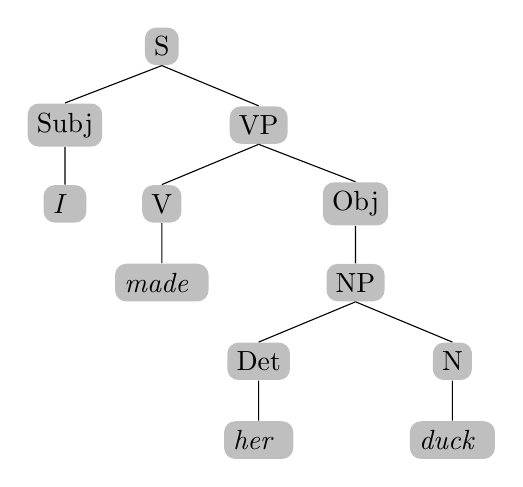
\begin{tikzpicture}[sibling distance=7em,
            level distance=1.0cm,
           every node/.style = {shape=rectangle, rounded corners,
             align=center, fill=black!25}]]
           \node {S}
             child { node {Subj}
               child { node {\textit{I} } } }
             child { node {VP}
               child { node {V}
                 child { node {\textit{made} } } }
               child { node {Obj}
                 child { node {NP}
                  child {node {Det} child { node {\textit{her} } } }
                  child {node {N} child { node { \textit{duck} } } } } } };
        \end{tikzpicture}

\end{enumerate}

\section*{Question 3}
\begin{enumerate}[label=(\alph*)]
    \item For every non-root we keep the highest incoming edge, from where we can see a cycle between the nodes of `plain', `bagels' and `likes':

        \tikzstyle{edge} = [draw,thick]
        \tikzstyle{weight} = [font=\small]
        \tikzstyle{selected edge} = [draw,line width=5pt,-,red!50]
        \pgfdeclarelayer{background}
        \pgfsetlayers{background,main}
        \begin{tikzpicture}[shorten >=1pt,->, auto]
        \tikzstyle{vertex}=[circle,fill=black!25, minimum size=37pt,inner sep=0pt]

            \foreach \name/\x/\y in {root/1/5, likes/5/2, John/5/5, bagels/3/0, plain/0/0}
            \node[vertex] (\name) at (\x,\y) {\name};

            \foreach \from/\to/\label in {likes/John/20, plain/likes/20, bagels/plain/15, likes/bagels/30}
                \path[edge] (\from) --  node [weight]{\label} (\to) ;

            \begin{pgfonlayer}{background}
                \foreach \source / \dest in {plain/likes, bagels/plain, likes/bagels}
                \path[selected edge] (\source.center) -- (\dest.center);
            \end{pgfonlayer}
        \end{tikzpicture}
        \vspace{2em}

    \item After completing the algorithm we result in:

        \begin{tikzpicture}[shorten >=1pt,->, auto]
        \tikzstyle{vertex}=[circle,fill=black!25, minimum size=37pt,inner sep=0pt]

            \foreach \name/\x/\y in {root/1/5, likes/5/2, John/5/5, bagels/3/0, plain/0/0}
            \node[vertex] (\name) at (\x,\y) {\name};

            \foreach \from/\to/\label in {root/likes/15, likes/John/20, bagels/plain/15, likes/bagels/30}
                \path[edge] (\from) --  node [weight]{\label} (\to) ;

        \end{tikzpicture}
\end{enumerate}

\section*{Question 4}

\begin{enumerate}[label=(\alph*)]

        \item

            We define a set $A$ as the set as created arcs, with initial value
            $A = \emptyset$. From this we start parsing according to Nivre's
            algorithm\footnote{An efficient algorithm for projective
            dependency parsing, Joakim Nivre, 2003}.

            \begin{table}[h]
                \centering
                \begin{tabular}{l|l|r|l}
                    Transition & Stack & Buffer & Arcs ($A$)\\
                    \hline
                    &  & A koala eats leafs and barks & $A$\\
                    SHIFT &   A & koala eats leafs and barks & $A$\\
                    LEFT-ARC(det) & & eats leafs and barks & $A = A \cup \text{det(koala, A)}$\\
                    SHIFT &  koala & eats leafs and barks & $A$\\
                    LEFT-ARC(nsubj) & eats & leafs and barks & $A = A \cup \text{nsubj(eats, koala)}$\\
                    RIGHT-ARC(dobj) &  eats leafs & and barks & $A$\\
                    RIGHT-ARC(cc) &  eats leafs and  & barks & $A =A \cup \text{cc(leafs, and)}$\\
                    REDUCE &  eats leafs & barks & $A$\\
                    RIGHT-ARC(conj) &  eats leafs barks & & $A=A\cup\text{conj(leafs, barks)}$\\
                    REDUCE &  eats leafs & & $A$\\
                    REDUCE &  eats & & $A$\\
                \end{tabular}
            \end{table}

            As our buffer is empty and there is only one word left on the
            stack, we see that the root of the sentence is ``eats''. We then
            add the root transition to $A$: $A = A\cup \text{root(root,
            eats)}$. This results in $A = \{\text{det(koala, A)},
            \text{nsubj(eats, koala)}, \text{dobj(eats, leafs)},
            \text{cc(leafs, and)}, \text{conj(leafs, barks)}, \text{root(root,
            eats)}\}$.

\end{enumerate}
\end{document}
% vim: ft=tex tw=0
